\setcounter{deso}{2}
\begin{name}
	{ÔN TẬP KIỂM TRA CUỐI HỌC KÌ 1 - tp2}
	{TOÁN 10}
	{LỚP TOÁN THẦY PHÁT}
	{\thoigian}
\end{name}
%================================PHẦN I
\caulc
\Opensolutionfile{ans}[ans/0-HK1-CD-2-SoBacGiang-2324-Phan-I]
\begin{ex}%[0H5N2-2]%[VN-MT6, Đào Trung Kiên]%[Sở Bắc Giang]
	Cho bốn điểm bất kì $A$, $B$, $C$, $O$. Đẳng thức nào sau đây đúng?
	\choice
	{$\overrightarrow{AB}=\overrightarrow{AC}+\overrightarrow{BC}$}
	{$\overrightarrow{OA}=\overrightarrow{OB}+\overrightarrow{AB}$}
	{\True $\overrightarrow{OA}=\overrightarrow{CA}+\overrightarrow{OC}$}
	{$\overrightarrow{AB}=\overrightarrow{OB}+\overrightarrow{OA}$}
	\loigiai
	{
		Ta có $\overrightarrow{OA}=\overrightarrow{OC}+\overrightarrow{CA}=\overrightarrow{CA}+\overrightarrow{OC}$.
	}
\end{ex}

\begin{ex}%[0D3N2-3]%[VN-MT6, Đào Trung Kiên]%[Sở Bắc Giang]
	Trục đối xứng của parabol $y=x^2-4x-5$ là
	\choice
	{$x=-2$}
	{$x=-4$}
	{$x=4$}
	{\True $x=2$}
	\loigiai
	{
		Trục đối xứng của parabol là $x=\dfrac{-(-4)}{2\cdot1}=2$.
	}
\end{ex}

\begin{ex}%[1D1N2-2]%[[0H4N1-2]%[VN-MT6, Đào Trung Kiên]%[Sở Bắc Giang]
	Trong các đẳng thức sau đây, đẳng thức nào đúng?
	\choice
	{$\cot 150^\circ=\sqrt 3$}
	{\True $\cos 150^\circ=-\dfrac{\sqrt 3}{2}$}
	{$\sin 150^\circ=-\dfrac{\sqrt 3}{2}$}
	{$\tan 150^\circ=\dfrac{\sqrt 3}{3}$}
	\loigiai
	{
		Ta có $\cos 150^\circ=-\dfrac{\sqrt 3}{2}$.
	}
\end{ex}

\begin{ex}%[0D1N1-3]%[VN-MT6, Đào Trung Kiên]%[Sở Bắc Giang]
	Mệnh đề phủ định của mệnh đề \lq\lq $\forall x\in\mathbb{R}$, $x^2-4x+5>0$\rq\rq\ là
	\choice
	{\lq\lq $\exists x\in\mathbb{R}$, $x^2-4x+5>0$\rq\rq}
	{\lq\lq $\forall x\in\mathbb{R}$, $x^2-4x+5\leq 0$\rq\rq}
	{\lq\lq $\exists x\in\mathbb{R}$, $x^2-4x+5<0$\rq\rq}
	{\True \lq\lq $\exists x\in\mathbb{R}$, $x^2-4x+5\leq 0$\rq\rq}
	\loigiai
	{
		Mệnh đề phủ định của mệnh đề \lq\lq $\forall x\in\mathbb{R}$, $x^2-4x+5>0$\rq\rq\ là \lq\lq $\exists x\in\mathbb{R}$, $x^2-4x+5\leq 0$\rq\rq.
	}
\end{ex}

\begin{ex}%[0D3N1-2]%[VN-MT6, Đào Trung Kiên]%[Sở Bắc Giang]
	Tập xác định của hàm số $y=\sqrt{x-1}+\sqrt{2-x}$ là
	\choice
	{\True $\mathscr{D}=[1;2]$}
	{$\mathscr{D}=(-\infty;1]\cup[2;+\infty)$}
	{$\mathscr{D}=(-\infty;1)\cup (2;+\infty)$}
	{$\mathscr{D}=(1;2)$}
	\loigiai
	{
		Điều kiện xác định của hàm số $y=\sqrt{x-1}+\sqrt{2-x}$ là $\heva{&x-1\geq 0\\&2-x\geq 0} \Leftrightarrow 1\leq x\leq 2$.\\
		Vậy tập xác định của hàm số $y=\sqrt{x-1}+\sqrt{2-x}$ là $\mathscr{D}=[1;2]$.
	}
\end{ex}

\begin{ex}%[0H4N2-1]%[VN-MT6, Đào Trung Kiên]%[Sở Bắc Giang]
	Cho tam giác $ABC$ có $AC=b$. Bán kính $R$ của đường tròn ngoại tiếp tam giác $ABC$ được tính bởi công thức nào sau đây?
	\choice
	{$R=\dfrac{2b}{\sin B}$}
	{\True $R=\dfrac{b}{2\sin B}$}
	{$R=\dfrac{\sin B}{b}$}
	{$R=\dfrac{\sin B}{2b}$}
	\loigiai
	{
		Ta có $\dfrac{b}{\sin B}=2R \Leftrightarrow R=\dfrac{b}{2\sin B}$.
	}
\end{ex}

\begin{ex}%[0D2N2-2]%[VN-MT6, Đào Trung Kiên]%[Sở Bắc Giang]
	\immini[thm]
	{Bất phương trình nào sau đây có miền nghiệm là phần \textbf{không} tô đậm (không kể đường thẳng $d$) như hình vẽ?
		\choice[2]
		{$3x-2y>-6$}
		{$3x-2y\geq -6$}
		{\True $3x-2y<-6$}
		{$3x-2y\leq -6$}
	}
	{\begin{tikzpicture}[scale=0.75, font=\footnotesize, line join=round, line cap=round, >=stealth]
			\draw[thick, ->](-3.5,0)--(1,0)node[below]{$x$};
			\draw[thick, ->](0,-1.5)--(0,4)node[left]{$y$};
			\fill[pattern=north west lines, pattern color = blue!70!white] (-3,-1.5)--(1,-1.5)--(1,4)--(2/3,4);
			\draw[smooth, samples=100, domain=-3:2/3]plot(\x,{3/2*(\x)+3});
			\fill[white]
			(-0.35,-0.35)circle(6.5pt)
			;
			\path
			(-0.35,-0.35)node[]{$O$}
			(-2.2,0)node[above]{$-2$}
			(0,3)node[left]{$3$}
			(-1,2)node[]{$d$}
			;
		\end{tikzpicture}
	}
	\loigiai
	{Ta thấy điểm $O(0;0)$ thuộc miền nghiệm của các bất phương trình $3x-2y>-6$ và $3x-2y\geq -6$. \\
		Do đó phần nửa mặt phẳng bờ $d$, không chứa điểm $O$ và không kể đường thẳng $d$ là miền nghiệm của bất phương trình $3x-2y< -6$.}
\end{ex}

\begin{ex}%[0H9N1-4]%[Dự án đề kiểm tra Toán khối 10 HKI NH23-24-Dot 15- Hồ Văn Trung]%[THPT Lê Qúy Đôn- TPHCM]
Trong mặt phẳng $Oxy$, cho $\overrightarrow{a}=\left(-5;0\right)$, $\overrightarrow{b}=\left(4;x\right)$. Tìm giá trị $x$ để hai vectơ $\overrightarrow{a}$ và $\overrightarrow{b}$ cùng phương.
\choice
{$x=-1$}
{\True $x=0$}
{$x=4$}
{$x=-5$}
\loigiai{Để hai vectơ $\vec{a}$, $\vec{b}$ cùng phương thì $-5 \cdot x = 0 \cdot 4 \Rightarrow x=0.$
}
\end{ex}

\begin{ex}%[0H4N2-1]%[VN-MT6, Đào Trung Kiên]%[Sở Bắc Giang]
	Cho tam giác $ABC$ có $AB=2$, $AC=3$ và $\widehat{BAC}=60^\circ$. Độ dài cạnh $BC$ là
	\choice
	{\True $\sqrt{7}$}
	{$\sqrt{19}$}
	{$7$}
	{$\sqrt{13}$}
	\loigiai
	{
		Ta có $BC=\sqrt{AB^2+AC^2-2\cdot AB\cdot AC\cdot\cos\widehat{BAC}}=\sqrt{2^2+3^2-2\cdot2\cdot3\cdot\dfrac{1}{2}}=\sqrt{7}$.
	}
\end{ex}

\begin{ex}%[0H5H4-1]%[VN-MT6, Đào Trung Kiên]%[Sở Bắc Giang]
	Cho tam giác đều $ABC$ có cạnh bằng $a$. Khẳng định nào sau đây đúng?
	\choice
	{$\overrightarrow{AB}\cdot\overrightarrow{BC}=-\dfrac{a^2\sqrt 3}{2}$}
	{$\overrightarrow{AB}\cdot\overrightarrow{BC}=\dfrac{a^2\sqrt 3}{2}$}
	{$\overrightarrow{AB}\cdot\overrightarrow{BC}=\dfrac{a^2}{2}$}
	{\True $\overrightarrow{AB}\cdot\overrightarrow{BC}=-\dfrac{a^2}{2}$}
	\loigiai
	{
		\begin{center}
			\begin{tikzpicture}[font=\footnotesize,line join=round, line cap=round, >=stealth,scale=1]
				\path
				(0,0) coordinate (B)
				(B)+(60:3) coordinate (A)
				(B)+(0:3) coordinate (C)
				;
				\draw (A)--(B)--(C)--cycle ;
				\foreach \x/\g in {A/90,B/180,C/0}\fill[draw,fill=black] (\x) circle (1pt)+(\g:3mm) node{$\x$};
			\end{tikzpicture}
			
		\end{center}
		Ta có $\overrightarrow{AB}\cdot\overrightarrow{BC}=-\overrightarrow{BA}\cdot\overrightarrow{BC}=-\left|\overrightarrow{BA}\right|\cdot\left|\overrightarrow{BC}\right|\cdot\cos\widehat{ABC}=-a\cdot a\cdot\cos 60^\circ=-\dfrac{a^2}{2}$.
	}
\end{ex}

\begin{ex}%[0H5N3-1]%[VN-MT6, Đào Trung Kiên]%[Sở Bắc Giang]
	Cho đoạn thẳng $AB$, gọi $M$ là trung điểm của $AB$. Đẳng thức vectơ nào sau đây đúng?
	\choice
	{$\overrightarrow{AM}=\overrightarrow{BM}$}
	{$\overrightarrow{AB}=2\overrightarrow{MA}$}
	{\True $\overrightarrow{AM}=\dfrac{1}{2}\overrightarrow{AB}$}
	{$\overrightarrow{AB}=2\overrightarrow{BM}$}
	\loigiai
	{
		Do $M$ là trung điểm $AB\Rightarrow \overrightarrow{AM}=\dfrac{1}{2}\overrightarrow{AB}$.
	}
\end{ex}

\begin{ex}%[0H9N2-1]
%Câu 9 :
Trong mặt phẳng tọa độ $Oxy$ cho ba điểm $A\left( 3;-1 \right),B\left( 2;10 \right),C\left( -4;2 \right)$. Tính tích vô hướng $\overrightarrow{AB}\cdot \overrightarrow{AC}$.
\choice
{\True $40$}
{$-40$}
{$26$}
{$-26$}
\loigiai{
Ta có \begin{eqnarray*}
\overrightarrow{AB}=\left( -1;11 \right);\;\overrightarrow{AC}=\left( -7;3 \right)
\Rightarrow \overrightarrow{AB}\cdot \overrightarrow{AC}=-1\cdot (-7)+11\cdot 3=40.
\end{eqnarray*}
}
\end{ex}

\Closesolutionfile{ans}
%================================PHẦN II
\cauds
\Opensolutionfile{ans}[ans/0-HK1-CD-2-SoBacGiang-2324-Phan-II]
% \setcounter{ex}{0}

\begin{ex}%[0D7H2-1]%[VN-MT6, Đào Trung Kiên]%[Sở Bắc Giang]
	Cho hàm số $y=f(x)=-x^2+3x-2$.
	\choiceTF
	{\True Tập nghiệm của bất phương trình $f(x)\geq 0$ là $[1;2]$}
	{\True Phương trình $f(x)=0$ có hai nghiệm phân biệt}
	{Giá trị lớn nhất của hàm số $f(x)$ bằng $\dfrac{3}{2}$}
	{Có duy nhất một giá trị nguyên dương của $m$ để phương trình $f(x)=m$ có hai nghiệm phân biệt}
	\loigiai
	{	\begin{itemchoice}
			\itemch \textbf{Đúng}.\\Ta có $-x^2+3x-2\geq 0 \Leftrightarrow 1\leq x\leq 2$.\\
			Vậy tập nghiệm của bất phương trình $-x^2+3x-2\geq 0$ là $[1;2]$. 
			\itemch \textbf{Đúng}.\\ $f(x)=0\Leftrightarrow -x^2+3x-2=0\Leftrightarrow \hoac{&x=1\\&x=2}$ nên phương trình có hai nghiệm phân biệt.
			\itemch \textbf{Sai}.\\ Ta có $f(x)=\dfrac{1}{4}-\left(x-\dfrac{3}{2}\right)^2\leq \dfrac{1}{4}$, đẳng thức xảy ra khi và chỉ khi $x=\dfrac{3}{2}$.\\
			Do đó giá trị lớn nhất của hàm số bằng $f\left(\dfrac{3}{2}\right)=\dfrac{1}{4}$.
			\itemch \textbf{Sai}.\\ Ta có đồ thị của hàm số $y=f(x)$ như sau
			\begin{center}
				\begin{tikzpicture}[line join=round, line cap=round,>=stealth,xscale=1,yscale=1.2]
					\tikzset{every node/.style={scale=0.9}}
					\draw[->] (-2.1,0)--(4.1,0) node[below left] {$x$};
					\draw[->] (0,-2.9)--(0,1.1) node[below left] {$y$};
					\draw (0,0) node [below left] {$O$};
					\draw [dashed] (1.5,0)node[below]{$\tfrac{3}{2}$}--(1.5,0.25)--(0,.25)node[left]{$\tfrac{1}{4}$} (0,-2)node[left]{$-2$};
					\begin{scope}
						\clip (-2,-2.9) rectangle (4.5,2);
						\draw[samples=200,domain=-1:4,smooth,variable=\x] plot (\x,{-1*(\x)^2+3*(\x)+-2});
					\end{scope}
				\end{tikzpicture}
			\end{center}
			Từ đồ thị ta thấy phương trình $f(x)=m$ có hai nghiệm phân biệt khi và chỉ khi $m<\dfrac{1}{4}$ nên không có giá trị nguyên dương nào của $m$ thỏa mãn yêu cầu bài toán.
		\end{itemchoice}
		
	}
\end{ex}

\begin{ex}%[VN-MT-6,Đào Trung Kiên]%[0H5H3-1]
	Cho tam giác $ABC$. Gọi $M$ và $N$ lần lượt là trung điểm của $AB$ và $AC$.
	\choiceTF
	{\True $\overrightarrow{AB}=2\overrightarrow{AM}$}
	{\True $\overrightarrow{CN}=-\dfrac{1}{2}\overrightarrow{AC}$}
	{\True $\overrightarrow{BC}=2\overrightarrow{AN}-\overrightarrow{AB}$}
	{$\overrightarrow{CA}+\overrightarrow{CB}=\dfrac{1}{2}\overrightarrow{CM}$}
	\loigiai{
		\begin{center}
			\begin{tikzpicture}[font=\footnotesize,line join=round, line cap=round, >=stealth,scale=1]
				\path
				(0,0) coordinate (B)
				(2,2) coordinate (A)
				(5,0) coordinate (C)
				($(B)!.5!(A)$) coordinate (M)
				($(A)!.5!(C)$) coordinate (N)
				;
				\draw (A)--(B)--(C)--cycle (C)--(M)--(N) ;
				\foreach \x/\g in {A/90,B/180,C/0,M/180,N/0}\fill[draw,fill=black] (\x) circle (1pt)+(\g:3mm) node{$\x$};
			\end{tikzpicture}
		\end{center}
		\begin{itemchoice}
			\itemch {\bf Đúng}.\\
			Vì $M$ là trung điểm của $AB$ nên $\overrightarrow{AB}=2\overrightarrow{AM}$.
			\itemch {\bf Đúng}.\\Vì $N$ là trung điểm của $AB$ nên $\overrightarrow{CN}=-\dfrac{1}{2}\overrightarrow{AC}$.
			\itemch {\bf Đúng}.\\ Vì $M$ và $N$ lần lượt là trung điểm của $AB$ và $AC$ nên $2\overrightarrow{AN}=\overrightarrow{AC}$. Do đó \[2\overrightarrow{AN}-\overrightarrow{AB}=\overrightarrow{AC}-\overrightarrow{AB}=\overrightarrow{BC}.\]
			\itemch {\bf Sai}.\\ Vì $M$ là trung điểm của $AB$ nên $\overrightarrow{CA}+\overrightarrow{CB}=2\overrightarrow{CM}$.
	\end{itemchoice}}	
\end{ex}

\Closesolutionfile{ans}
%================================PHẦN III
\caukq
\Opensolutionfile{ans}[ans/0-HK1-CD-2-SoBacGiang-2324-Phan-III]
% \setcounter{ex}{0}

\begin{ex}%[0D7H2-1]%[VN-MT6, Đào Trung Kiên]%[Sở Bắc Giang]
	Bất phương trình $-x^2+3x-2\geq 0$ có bao nhiêu nghiệm nguyên dương?
	\shortans[]{$2$}
	\loigiai
	{Xét phương trình $-x^2+3x-2=0\Leftrightarrow \hoac{x=1\\x=2.}$\\
		Từ đó ta có bảng xét dấu sau của $f(x)=-x^2+3x-2$ như sau
		\begin{center}
			
\begin{tikzpicture}
				\tkzTabInit[nocadre=true, lgt=1.2, espcl=3.5, deltacl=0.5]
				{$x$/0.7,$f(x)$/0.7}
				{$-\infty$,$1$,$2$,$+\infty$}
				\tkzTabLine{,-,0,+,0,-}
			\end{tikzpicture}
		\end{center}
		Vậy tập nghiệm của bất phương trình $-x^2+3x-2\geq 0$ là $[1;2]$ nên bất phương trình có hai nghiệm nguyên dương.
	}
\end{ex}

\begin{ex}%[0H4V2-1]%[VN-MT6, Đào Trung Kiên]%[Sở Bắc Giang]
	\immini[thm]{Trên bản đồ địa lý người ta thường gọi tứ giác với $4$ đỉnh lần lượt là các thành phố Hà Tiên, Châu Đốc, Long Xuyên, Rạch Giá là tứ giác Long Xuyên. Dựa vào các khoảng cách đã cho trên hình vẽ, ta tính được khoảng cách giữa Châu Đốc và Rạch Giá gần đúng bằng (làm tròn đến hàng đơn vị)
		% \choice[2]
		% {$80$ km}
		% {\True $76$ km}
		% {$120$ km}
		% {$70$ km}
	}
	{\begin{tikzpicture}[scale=0.55, font=\footnotesize, line join=round, line cap=round, >=stealth]
			\path
			(0,0)coordinate(H)node[left]{$H$}
			(9,0)coordinate(L)node[right]{$L$}
			(6.2,3)coordinate(C)node[above]{$C$}
			(5.8,-2.9)coordinate(R)node[below]{$R$}
			(0,-0.7)node[]{Hà Tiên}
			(10.5,-0.7)node[]{Long Xuyên}
			(5.8,-4.2)node[]{Rạch Giá}
			(6.2,4.3)node[]{Châu Đốc}
			($(H)!0.5!(C)$)node[above, rotate=30]{$78$ km}
			($(C)!0.5!(L)$)node[above, rotate=-45]{$49$ km}
			($(L)!0.6!(R)$)node[below, rotate=45]{$56$ km}
			($(R)!0.4!(H)$)node[below, rotate=-30]{$77$ km}
			($(H)!0.5!(L)$)node[above]{$104$ km}
			($(C)!0.7!(R)$)node[right]{?}
			;
			\draw(H)--(C)--(L)--(R)--(H)--(L);
			\draw[dashed](C)--(R);
		\end{tikzpicture}
	}
	\shortans{76}
	\loigiai
	{Xét tam giác $HCL$ ta có $\cos\widehat{CLH}=\dfrac{CL^2+HL^2-CH^2}{2CL\cdot HL}=\dfrac{1\,019}{1\,456} \Rightarrow \widehat{CLH}\approx45{,}58^{\circ}$.\\
		Xét tam giác $RHL$ ta có $\cos\widehat{RLH}=\dfrac{RL^2+HL^2-RH^2}{2RL\cdot HL}=\dfrac{8\,023}{11\,648} \Rightarrow \widehat{RLH}\approx46{,}47^{\circ}$.\\
		Do đó $\widehat{CLR}=\widehat{CLH}+\widehat{RLH}\approx92{,}05^{\circ}$.\\
		Xét tam giác $RLC$ ta có $CR^2=CL^2+LR^2-2\cdot CL\cdot LR\cdot \cos \widehat{CLR}\approx 5\,733{,}3\Rightarrow CR\approx 76$ (km).\\
		Vậy khoảng cách giữa Châu Đốc và Rạch Giá gần đúng bằng $76$ km.
	}
\end{ex}

\begin{ex}%[0D2V2-3]%[VN-MT6, Đào Trung Kiên]%[Sở Bắc Giang]
	Trong một cuộc thi pha chế, mỗi đội chơi được sử dụng tối đa $12$ gam hương liệu hòa tan, $9$ lít nước và $315$ gam đường để pha chế hai loại nước A và B. Để pha chế $1$ lít nước loại A cần $45$ gam đường, $1$ lít nước và $0,5$ gam hương liệu. Để pha chế $1$ lít nước loại B cần $15$ gam đường, $1$ lít nước và $2$ gam hương liệu. Mỗi lít nước loại A nhận được $60$ điểm thưởng, mỗi lít nước loại B nhận được $80$ điểm thưởng. Để đội chơi được số điểm thưởng là lớn nhất thì cần pha chế $a$ lít nước loại A và $b$ lít nước loại B. Tính tổng $a+b$.
	\shortans[]{$9$}
	\loigiai
	{Gọi $x$, $y$ lần lượt là số loại nước A và nước B mà đội chơi cần pha chế. \\
		Vì mỗi đội chơi được sử dụng tối đa $12$ gam hương liệu hòa tan nên ta có $0{,}5x+2y\leq 12$.\\
		Mỗi đội chơi được sử dụng tối đa $9$ lít nước nên ta có $x+y\leq 9$.\\
		Mỗi đội được sử dụng tối đa $315$ gam đường nên ta có bất phương trình $45x+15y\leq 315$.\\
		Từ đó ta có $\heva{&x\geq 0\\&y\geq 0\\ & 0{,}5x+2y\leq 12 \\ &x+y\leq 9 \\ & 45x+15y\leq 315} \Leftrightarrow \heva{&x\geq 0\\ &y\geq 0\\ &x+4y\leq 24\\ &x+y\leq 9\\ &3x+y\leq 21.}$ \hfill $(1)$ \\
		Số điểm thưởng là $f(x,y)=60x+80y$.\\
		\begin{center}
			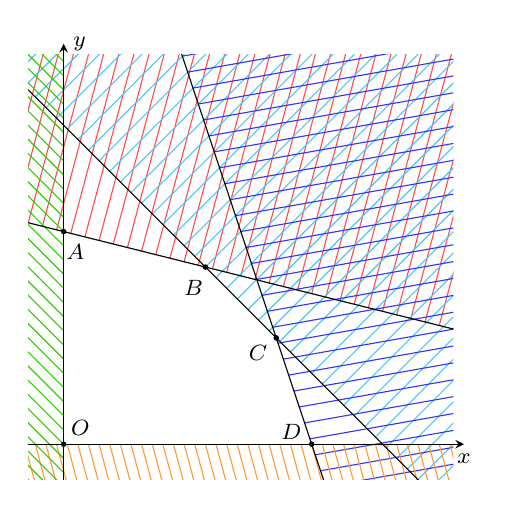
\begin{tikzpicture}[scale=1, font=\footnotesize, line join=round, line cap=round, >=stealth, x=0.45cm, y=0.45cm]
				\tikzset{declare function={f(\x)=6-0.25*(\x); g(\x)=9-\x; h(\x)=21-3*(\x);}}
				\def\xt{-1} \def\xp{11}
				\def\yd{-1} \def\yt{11}
				\begin{scope}
					\clip (\xt,\yd) rectangle (\xp,\yt);
					\foreach \i in {-3,-2.6,...,\xp} \draw[red!70!white] (\i,{f(\i)})--++(75:8);
					\foreach \j in {-2,-1.7,...,\xp} \draw[cyan!70!white] (\j,{g(\j)})--++(45:10);
					\foreach \k in {-1,-0.85,...,\xp} \draw[blue!80!white] (\k,{h(\k)})--++(10:8);
					\foreach \x in {-2,-1.7,...,\xp} \draw[orange!80!white] (\x,0)--++(-75:2);
					\foreach \y in {-2,-1.6,...,\yt} \draw[green!80!red] (0,\y)--++(135:2);
					\draw[domain=\xt:\xp] plot(\x,{f(\x)})
					plot(\x,{g(\x)})
					plot(\x,{h(\x)});
				\end{scope}	
				\draw[->] (\xt,0)--(\xp+0.3,0)node[below]{$x$};
				\draw[->] (0,\yd)--(0,\yt+0.3)node[right]{$y$};
				\foreach \p/\n/\g in {(0,0)/O/45, (0,6)/A/-60, (4,5)/B/-120, (6,3)/C/220, (7,0)/D/150} \fill \p node[shift={(\g:3mm)}]{$\n$} circle(1pt);
			\end{tikzpicture}
		\end{center}
		Miền nghiệm của hệ bất phương trình $(1)$ là ngũ giác $OABCD$ với $A(0;6)$; $O(0;0)$; $B(4;5)$, $C(6;3)$, $D(7;0)$. \\
		Vì giá trị lớn nhất của $f(x;y)=60x+80y$ đạt được tại đỉnh của miền nghiệm.\\
		Ta có $f(0;0)=0$, $f(0;6)=480$, $f(4;5)=640$, $f(6;3)=600$, $f(7;0)=420$.\\
		Suy ra $f(x,y)$ đạt giá trị lớn nhất tại $B(4; 5)$.\\
		Vậy để đạt số điểm thưởng lớn nhất đội chơi cần pha chế $9$ lít nước gồm $4$ lít nước loại A và $5$ lít nước loại B. 
	}
\end{ex}

\begin{ex}%[0D1V3-5]
Trường THPT Tài Đức tổ chức cho học sinh học thể dục dưới hình thức Câu lạc bộ, các học sinh đăng kí môn thể thao mà bản thân yêu thích. Lớp $10$A của trường có $24$ học sinh đăng kí môn bóng đá, $20$ học sinh đăng kí môn cầu lông, $7$ học sinh đăng kí cả hai môn bóng đá và cầu lông, $8$ học sinh đăng kí một môn khác. Hỏi sỉ số của lớp $10$A là bao nhiêu?
\shortans[4]{$45$}
\loigiai{
\begin{itemize}
\item Số học sinh chỉ đăng kí môn bóng đá là $24-7=17$ học sinh.
\item Số học sinh chỉ đăng kí môn cầu lông là $20-7=13$ học sinh.
\item Sĩ số của lớp 10A là $17+13+7+8=45$ học sinh.
\end{itemize}
}
\end{ex}
\Closesolutionfile{ans}
% \begin{indapan}
% 	{ans/0-HK1-CD-2-SoBacGiang-2324}
% \end{indapan}


\TL
\begin{ex}%[0D7H3-2]
	Giải phương trình
	\begin{enumerate}
		\item $2\sqrt{x+3}=\sqrt{x^2-4x+19}$
		\item $\sqrt{3x^2+24x+22}-2x=1$
	\end{enumerate}  
	\loigiai{
	\begin{enumerate}
		\item $2\sqrt{x+3}=\sqrt{x^2-4x+19} $
		Bình phương hai vế ta được
		\[4(x+3)=x^2-4x+19 \Leftrightarrow x^2-8x+7=0 \Leftrightarrow \hoac{&x=1\\&x=7.}\]
		Thay vào phương trình ban đầu kiểm tra, ta thấy cả hai nghiệm đều thoả mãn. \\
		Vậy phương trình $2\sqrt{x+3}=\sqrt{x^2-4x+19}$ có hai nghiệm là $x=1$ và $x=7$.
		\item $\sqrt{3x^2+24x+22}-2x=1 \Leftrightarrow \sqrt{3x^2+24x+22}=1+2x$. \\
		Bình phương hai vế của phương trình trên ta được
		\[3x^2+24x+22=\left(1+2x\right)^2 \Leftrightarrow x^2-20x-21=0 \Leftrightarrow \hoac{&x=21\\&x=-1.}\]
		Thay vào phương trình ban đầu kiểm tra, ta thấy chỉ có $x=21$ thỏa mãn. \\
		Vậy phương trình $\sqrt{3x^2+24x+22}-2x=1$ có nghiệm duy nhất là $x=21$.
	\end{enumerate}
	}
\end{ex}

\begin{ex}%[0H4V2-1]%[VN-MT6, Đào Trung Kiên]%[Sở Bắc Giang]
	Cho tam giác $ABC$ có $AB=6$ cm, $AC=8$ cm và $\widehat{A}=60^\circ$. Gọi $M$ là trung điểm của $BC$. Qua $B$ kẻ một đường thẳng vuông góc với $AM$, cắt $AC$ tại $N$. Tính tỉ số $\dfrac{AN}{AC}$ (làm tròn kết quả đến hàng phần trăm).
	% \shortans[]{$0{,}68$}
	\loigiai{
		\begin{center}
			\begin{tikzpicture}[scale=1, font=\footnotesize, line join=round, line cap=round, >=stealth]
				\path
				(0,0) coordinate (A)
				($(A)+(60:3)$) coordinate (B)
				($(A)+(0:4)$) coordinate (C)
				($(C)!0.5!(B)$)coordinate(M)
				($(A)!(B)!(M)$)coordinate(K)
				(intersection of B--K and A--C)coordinate(N);
				\draw(A)--(B)--(N) (B)--(C) (C)--(A)--(M);
				\foreach \p/\q in {B/90, A/190, C/-30, M/30, N/-90} \fill (\p) circle (1pt) ($(\p)+(\q:2.5mm)$) node{$\p$};
			\end{tikzpicture}
		\end{center}	
		Do $N$ thuộc $AC$ nên ta có $\overrightarrow{AN}=k\overrightarrow{AC} \Rightarrow \overrightarrow{BN}=\overrightarrow{AN}-\overrightarrow{AB} =-\overrightarrow{AB}+k\overrightarrow{AC}$.\\
		Vì $BN\perp AM$ nên ta có $\overrightarrow{BN}\cdot \overrightarrow{AM}=0$.\\
		Mà $\overrightarrow{AM}=\dfrac{1}{2}\left(\overrightarrow{AB}+\overrightarrow{AC}\right)$ và $\overrightarrow{AB}\cdot \overrightarrow{AC} = AB\cdot AC \cdot \cos\widehat{BAC} = 24$ nên
		\begin{eqnarray*}
			\overrightarrow{BN}\cdot \overrightarrow{AM}=0&\Leftrightarrow& \left(-\overrightarrow{AB}+k\overrightarrow{AC}\right)\left(\overrightarrow{AB}+\overrightarrow{AC}\right)=0\\
			&\Leftrightarrow& -\overrightarrow{AB}^2-\overrightarrow{AB}\cdot\overrightarrow{AC}+k\overrightarrow{AB}\cdot\overrightarrow{AC}+k\overrightarrow{AC}^2=0\\
			&\Leftrightarrow& -36-24+24k+64k=0\\
			&\Leftrightarrow &k=\dfrac{15}{22}.
		\end{eqnarray*}
		Suy ra $\overrightarrow{AN}=\dfrac{15}{22}\overrightarrow{AC}\Rightarrow AN=\dfrac{15}{12}AC$.\\
		Vậy $\dfrac{AN}{AC}=\dfrac{15}{22}\approx 0{,}68$.
	}
\end{ex}

\begin{ex}%[10-11-12EX-HK1-2425]%[Lê Quốc Hiệp]%[0D7V2-7]
Lợi nhuận $T(x)$ của một cơ sở sản xuất khi bán hết $x$ sản phẩm trang trí trong một tuần theo công thức $T(x)=-x^2+40x-309$ với đơn vị tính bằng triệu đồng. Nếu muốn lợi nhuận không dưới $10$ triệu đồng thì số sản phẩm ít nhất của cơ sở sản xuất trong một tuần là bao nhiêu? Biết rằng số sản phẩm được làm ra đều bán hết trong tuần đó.
% \shortans[oly]{$11$}
\loigiai
{
Điều kiện để lợi nhuận không dưới $10$ triệu đồng là
\begin{eqnarray*}
& & T(x) \geq 10\\
& \Leftrightarrow & -x^2+40x-309 \geq 10\\
& \Leftrightarrow & -x^2+40x-319 \geq 0\\
& \Leftrightarrow & 11 \leq x \leq 29.
\end{eqnarray*}
Vậy số sản phẩm ít nhất để đảm bảo lợi nhuận không dưới $10$ triệu đồng là $11$ sản phẩm.
}
\end{ex}